\section{The P\'olya density as an extreme value law}\label{ev:sec:decomp}

Write
\[
\Phi(u) = \sum_{n\ge1}\phi_n(u), \qquad \phi_n(u) = \left(2\pi^2n^4e^{9u} - 3\pi n^2e^{5u}\right)e^{-\pi n^2e^{4u}},
\]
so that $H(z) = \int_0^\infty\Phi(u)\cos(zu)\,du = \tfrac18\Xi(z/2)$ (checked numerically to $10^{-88}$ at $z=0$ and to $10^{-60}$ at $z=150+150i$). In Sections~\ref{ev:sec:decomp} to \ref{ev:sec:string} the kernel $\Phi$ is this one, the kernel $\Phi_{\mathrm{dBN}}$ of Section~\ref{ch:dbn} in the normalisation of Rodgers and Tao, not that of \eqref{eq:ch2:Phi}; the zeros of $H$ are at $z=\pm2\gamma_k$, and $x=z/2$ is the variable of the zeros. Let $g_k(x) = e^{-kx}\exp(-e^{-x})/\Gamma(k)$, the density of $-\log G_k$ for a gamma variable $G_k$ of shape $k$: for integer $k$ the law of the $k$th largest point of the Gumbel limit process with intensity $e^{-x}dx$, for real $k$ a fractional order statistic in the sense of Stigler \cite{Stigler77}. Proposition~\ref{mw:prop:sum} and Section~\ref{ht:sec:ev} treat the maximum and the Gumbel law; here the individual terms of the theta series are decomposed.
% UNCHECKED: Stigler77, the statement is the source's and the paper was not read for this book.

\begin{theorem}[Gumbel decomposition]\label{ev:thm:decomp}
With $x = -4u - \log(\pi n^2)$, as densities in $x$,
\[
\phi_n(u)\,du = \pi^{-1/4}n^{-1/2}\Gamma(\tfrac54)\left[\tfrac58 g_{9/4}(x) - \tfrac34 g_{5/4}(x)\right]dx .
\]
The signed masses of the terms are $-\tfrac18\pi^{-1/4}\Gamma(\tfrac54)n^{-1/2}$, and the formal sum of the masses, regularised by $\zeta$, is
\[
-\tfrac18\pi^{-1/4}\Gamma(\tfrac54)\zeta(\tfrac12) = \tfrac14\xi(\tfrac12) = \int_\R\Phi .
\]
With $s = (1+iz)/2$,
\[
\int_\R\phi_n(u)e^{izu}du = \tfrac14 n^{-s}\xi(s)/\zeta(s).
\]
\end{theorem}

\begin{proof}
Put $y=e^{-x}=\pi n^2e^{4u}$, so that $e^{9u}=(y/\pi n^2)^{9/4}$, $e^{5u}=(y/\pi n^2)^{5/4}$ and $du=-dx/4$. The coefficients become $2\pi^2n^4(\pi n^2)^{-9/4}=2\pi^{-1/4}n^{-1/2}$ and $3\pi n^2(\pi n^2)^{-5/4}=3\pi^{-1/4}n^{-1/2}$, and $\Gamma(\tfrac94)=\tfrac54\Gamma(\tfrac54)$ turns $\tfrac14\cdot2\Gamma(\tfrac94)$ into $\tfrac58\Gamma(\tfrac54)$. The masses are $\tfrac58-\tfrac34=-\tfrac18$ times the common factor. The $\zeta$ regularised sum is a formal identity (the series $\sum n^{-1/2}$ diverges), and it agrees with $\int_\R\Phi=\xi(\tfrac12)/4$ because $\Gamma(\tfrac54)=\tfrac14\Gamma(\tfrac14)$ and $\xi(\tfrac12)=-\tfrac18\pi^{-1/4}\Gamma(\tfrac14)\zeta(\tfrac12)$. For the transform, the same substitution gives $(\pi n^2)^{-iz/4}$ times a combination of $\Gamma(w)$ at $w=(9+iz)/4$ and $(5+iz)/4$, which equals $n^{-s}\pi^{-s/2}s(s-1)\Gamma(s/2)/8$.
\end{proof}

So the Dirichlet series of $\zeta$ is a sum over translates of one Gumbel kernel along the lattice $\tfrac12\log n$. The tail of the normalised law $p=4\Phi/\xi(\tfrac12)$ is $S(u)\sim(2\pi/\xi(\tfrac12))e^{5u}\exp(-\pi e^{4u})$ (proved, one integration), so $p$ is in the Gumbel domain of attraction of the theorem of Fisher, Tippett and Gnedenko (Proposition~\ref{mw:prop:gnedenko}). That the maximum of $N$ independent copies converges at the slow rate $1/\log N$ is a heuristic by analogy with the normal law, not used. Three families of approximations follow.

\begin{itemize}
\item \textit{Folded Gumbel.} $\Phi^F_N(u) = \sum_{n\le N}\phi_n(|u|)$. The sharp cutoff of the theta series at $N$ is the omitted set $\{n>N\}$ of Chapter~\ref{chap:miyatake} (Section~\ref{mi:sec:approx}), and the cosine transform of $\Phi^F_N$ is
\[\begin{aligned}H^F_N(z) &= \tfrac12\left[F_N(z)+F_N(-z)\right],\\ F_N(z)&=\sum_{n\le N}\Big[\tfrac12 a_n^{2-w_9}\Gamma(w_9,a_n) - \tfrac34 a_n^{1-w_5}\Gamma(w_5,a_n)\Big],\end{aligned}\]
where $a_n = \pi n^2$, $w_j = (j+iz)/4$ and $\Gamma(w,a)$ is the upper incomplete gamma function. For real $z$ this is $\operatorname{Re}F_N(z)$, but off the real axis only the symmetrised form is the transform of $\Phi^F_N$.
\item \textit{Two sided Gumbel.} P\'olya's kernel of Section~\ref{ch:biane} (equation~\eqref{eq:biane:P}),
\[\Phi^P(u) = (4\pi^2\cosh9u - 6\pi\cosh5u)e^{-2\pi\cosh4u}.\]
Here $e^{-2\pi\cosh4u}=\mathbb{P}(V\le u<W)$ for independent variables $V$ and $W$ with $\mathbb{P}(V\le u)=\exp(-\pi e^{-4u})$ and $\mathbb{P}(W>u)=\exp(-\pi e^{4u})$, a Gumbel maximum and a Gumbel minimum, and for real $z$
\[H^P(z) = \operatorname{Re}\left[\pi^2K_{(9+iz)/4}(2\pi) - \tfrac{3\pi}{2}K_{(5+iz)/4}(2\pi)\right].\]
\item \textit{Dyck chain.} With $H_n$ the height of a uniform Dyck path of length $2n$ and
\[Y_n = \sqrt{2/\pi}\,H_n/\sqrt{2n},\]
the Dirichlet polynomial $F_n(s) = \E[Y_n^s]$ tends to $2\xi(s)$ on $\operatorname{Re}s>0$, because $\E[Y^s] = 2\xi(s)$ for $Y=\sqrt{2/\pi}$ times the maximum of a Brownian excursion (Biane, Pitman and Yor \cite{BPY01}; this is $e^Y$ of Proposition~\ref{mw:prop:sum}) and the Dyck height scales to the excursion maximum (the height law of Dyck paths is in de Bruijn, Knuth and Rice \cite{deBruijnKnuthRice72}).
% UNCHECKED: deBruijnKnuthRice72, the statement is the source's and the paper was not read for this book.
% UNCHECKED: locally uniform convergence of E[Y_n^s] to 2 xi(s) on Re s > 0 needs uniform integrability of the moments of H_n/sqrt(2n); it is stated as in the source and was not proved or recomputed here. Conjecture ev:conj:lbias would imply it.
\end{itemize}

By \cite{BPY01} the normalised law $p$ is the law of $\tfrac12\log Y$ under the measure with density proportional to $Y^{1/2}$: indeed $\E[Y^{1/2}Y^{iz/2}]/\E[Y^{1/2}]=\xi(s)/\xi(\tfrac12)$. The Dyck chain is a Markov chain whose extremes arrive in clusters rather than as independent exceedances, as in the stationary chains of Smith, Tawn and Coles \cite{SmithTawnColes97} (the analogy is ours). Table~\ref{ev:tab:approx} lists the zeros of the approximations. The zero counts are sign changes of $H^F_N(2x)$, with signs certified on a grid of mesh $0.05$.
% UNCHECKED: SmithTawnColes97, the statement is the source's and the paper was not read for this book.

\begin{table}[h]\centering\footnotesize\setlength{\tabcolsep}{3pt}
\begin{tabular}{p{0.3\textwidth}p{0.3\textwidth}p{0.34\textwidth}}
\toprule
approximation & real zeros & accuracy\\
\midrule
folded, $N=2$ & 7 below $x=70$ & $3.9\cdot10^{-5}$ to $\gamma_3$\\
folded, $N=3$ & 15 below $x=100$ & $9.6\cdot10^{-6}$ to $\gamma_{11}$\\
folded, $N=4$ & 31 below $x=140$ & $5.8\cdot10^{-6}$ to $\gamma_{25}$\\
two sided (P\'olya) & all real & first zero $x=7.604$ against $\gamma_1=14.135$\\
Dyck chain, $n = 12800$ & zero near $\gamma_1$ off the line & $0.4367 + 14.0457i$ against $0.5 + 14.1347i$\\
Dyck chain, Richardson in $n^{-1/2}$ & off the line, to $10^{-3}$ & $0.50003 + 14.13473i$ (two steps)\\
\bottomrule
\end{tabular}
\caption{Zeros of the extreme value approximations (computed). For the Dyck chain the real parts of the zero near $\gamma_1$ for $n=800,\allowbreak1600,\allowbreak3200,\allowbreak6400,\allowbreak12800,\allowbreak25600$ are $0.2438,0.3196,0.3729,0.4103,0.4367,0.4553$, and the extrapolation uses $n=3200,\allowbreak6400,\allowbreak12800$.}\label{ev:tab:approx}
\end{table}

The folded family is accurate up to a height $T_N\approx4(N+1)^2$ in $x$ and then fails, because of a kink at the origin. Write $R_N=\Phi-\Phi^F_N=\sum_{n>N}\phi_n$ on $u\ge0$ and $\kappa_N=|R_N'(0)|$, the one sided slope. Its Fourier tail is of order $\kappa_N/z^2$, which overtakes $H(z)\approx|z|^{7/4}e^{-\pi z/8}$ when $x\approx4(N+1)^2$ (heuristic: a balance of leading orders). The slope is $\kappa_N=8.27\cdot10^{-8}$, $1.39\cdot10^{-16}$ and $2.87\cdot10^{-28}$ for $N=2,3,4$ (computed); the leading order formula $8\pi^3(N+1)^6e^{-\pi(N+1)^2}$ overstates it by $15\%$, $8\%$ and $5\%$. The predicted heights are $36$, $64$ and $100$. Measured by the first error above $10^{-2}$ in a tracked zero the breakdown is at $\gamma_5=32.9$, $\gamma_{15}=65.1$ and $\gamma_{30}=101.3$, and measured by the last real zero tracked it is at $x=39.5$, $65.0$ and $103.7$ (computed); with error thresholds from $10^{-3}$ to $10^{-1}$ the heights lie in $30$ to $38$, $59$ to $65$ and $96$ to $104$, so the rule is a statement about the order of magnitude and the leading constant, not a sharp threshold.

\begin{resultpar}\label{ev:res:dyckcensus}For the census of complex zeros below, the exact law of the height $H_n$ of the Dyck chain is used: by the reflection principle the number of Dyck paths of length $2n$ and height at most $h$ is $\sum_{k\in\mathbb Z}\big[\binom{2n}{n+k(h+2)}-\binom{2n}{n-1+k(h+2)}\big]$, out of $\binom{2n}{n}/(n+1)$. At $n=25600$, with these probabilities as balls at $256$ bits, the argument principle on the boundary of $-4<\operatorname{Re}s<6$, $0<\operatorname{Im}s<60$ counts $13$ zeros of the Dirichlet polynomial $F_n$ of the Dyck chain, in the bands $0<\operatorname{Im}s<20$, $20<\operatorname{Im}s<40$ and $40<\operatorname{Im}s<60$ the numbers $1$, $5$ and $7$ that the ordinates $\gamma_k$ have (the number of $\gamma_k$ below $60$ is $13$). There is no zero with $\tfrac12<\operatorname{Re}s<6$ and $0<\operatorname{Im}s<60$, and the real parts of the $13$ zeros run from $0.0907$ (the highest, at height $59.126$) to $0.4553$ (the lowest, at height $14.072$). Followed in $n$ from $25600$ through $12800$, $6400$ and $3200$ down to $1600$, with Newton's method started at the zero found for the next larger $n$, these $13$ zeros stay distinct and to the left of the line, and the zero of lowest height lies at distance $0.3082$, $0.1544$ and $0.0773$ from $\tfrac12+i\gamma_1$ for $n=1600$, $6400$ and $25600$ (computed). The count is for $n=25600$ only: at $n=1600$ the same contour holds $14$ zeros, and Newton's method started at $\tfrac12+i\gamma_k$ does not stay near it for $k=4,\dots,12$ (the starts $k=7$ and $8$ converge to one zero), so the zeros are identified by following them in $n$. This paragraph is based on \cite{P26excursion}.\end{resultpar}

The side from which these zeros approach is set by the lattice. By de Bruijn, Knuth and Rice \cite{deBruijnKnuthRice72}, $\E H_n=\sqrt{\pi n}-\frac32+o(1)$, while $\sqrt{2n}$ times the mean of the excursion maximum $\sqrt{\pi/2}\,Y$ is $\sqrt{\pi n}$; so to first order $H_n/\sqrt{2n}$ is that maximum moved down by
\[
\delta_n=\frac3{2\sqrt{2n}} .
\]
Heuristically, the reflection formula makes $\mathbb P(H_n\le h)$ close to $\mathbb P(\sqrt{\pi n}\,Y\le h+2)$, so that $H_n$ behaves like $\sqrt{\pi n}\,Y-2$ rounded up, which adds $\frac12$ on average. For the moments this reads as follows; since $\E Y^{s-1}=2\xi(s-1)$, it says that $F_n(s)$ is $\E(Y-\sqrt{2/\pi}\,\delta_n)^s$ to first order.
% UNCHECKED: deBruijnKnuthRice72, as in the Dyck chain item above.

\begin{conjecture}\label{ev:conj:lbias}
Uniformly on every compact subset of $\operatorname{Re}s>0$,
\[
F_n(s)=2\xi(s)-\frac{3s}{\sqrt{\pi n}}\,\xi(s-1)+O\Big(\frac1n\Big).
\]
\end{conjecture}

At $s=1$ the conjecture says $\E H_n=\sqrt{\pi n}-\frac32+O(n^{-1/2})$, which agrees with de Bruijn, Knuth and Rice, and it implies that $F_n\to2\xi$ locally uniformly on $\operatorname{Re}s>0$. Status: open; the zeros below agree with its consequence, Proposition~\ref{ev:prop:lbias} (computed).

\begin{proposition}\label{ev:prop:lbias}
Assume Conjecture~\ref{ev:conj:lbias}. Let $\rho$ be a simple zero of $\xi$ and put
\[
c_{\rm D}(\rho)=\sqrt{\frac2\pi}\,\frac{\rho\,\xi(\rho-1)}{\xi'(\rho)}=\sqrt{\frac2\pi}\,\frac{\rho\,\xi(2-\rho)}{\xi'(\rho)} .
\]
There is a constant $C$ such that for all large $n$, $F_n$ has exactly one zero $z_n(\rho)$ in the disc $|s-\rho-\delta_nc_{\rm D}(\rho)|<C/n$; thus $z_n(\rho)=\rho+\delta_nc_{\rm D}(\rho)+O(1/n)$. Status: conditional.
\end{proposition}

\begin{proof}
Put $g(s)=s\,\xi(s-1)$. On a closed disc about $\rho$ in $\operatorname{Re}s>0$, the conjecture and Taylor's formula give $F_n(s)=2\xi'(\rho)(s-\rho)-\frac3{\sqrt{\pi n}}\,g(\rho)+O\big(|s-\rho|^2+n^{-1/2}|s-\rho|+n^{-1}\big)$. Since $\frac{3g(\rho)}{2\sqrt{\pi n}\,\xi'(\rho)}=\delta_nc_{\rm D}(\rho)$, on the circle $|s-\rho-\delta_nc_{\rm D}(\rho)|=C/n$, where $|s-\rho|=O(n^{-1/2})$, this is $2\xi'(\rho)\big(s-\rho-\delta_nc_{\rm D}(\rho)\big)+O(1/n)$. The linear term has modulus $2|\xi'(\rho)|C/n$, which exceeds the error once $C$ is large, and Rouch\'e's theorem gives exactly one zero inside, as in Proposition~\ref{rz:prop:firstorder}. The second form of $c_{\rm D}$ is the functional equation.
\end{proof}

\begin{proposition}\label{ev:prop:lbphase}
Let $\rho=\frac12+i\gamma$, $\gamma>0$, be a simple zero on the critical line, with $\theta$ and $Z$ as in Theorem~\ref{rz:thm:kappaexact}. Then
\[
c_{\rm D}(\rho)=-\frac{C_{\rm D}(\gamma)\,e^{-i\Theta(\gamma)}}{Z'(\gamma)},\qquad C_{\rm D}(\gamma)=\frac{\sqrt2}\pi\,\Big|\frac32-i\gamma\Big|\,\Big|\frac{\Gamma(\frac34+\frac{i\gamma}2)}{\Gamma(\frac14+\frac{i\gamma}2)}\Big|\,\big|\zeta(\tfrac32+i\gamma)\big|>0,
\]
\[
\Theta(\gamma)=\theta(\gamma)+\arctan\tanh\frac{\pi\gamma}2+\arg\zeta(\tfrac32+i\gamma)-\arctan\frac3{2\gamma},
\]
so that $\operatorname{Re}c_{\rm D}(\rho)$ has the sign of $-\cos\Theta(\gamma)/Z'(\gamma)$. Status: proved.
\end{proposition}

\begin{proof}
Since $\Xi(t)=\xi(\frac12+it)=-\frac12(t^2+\frac14)\pi^{-1/4}|\Gamma(\frac14+\frac{it}2)|Z(t)$ and $Z(\gamma)=0$, $\xi'(\rho)=-i\,\Xi'(\gamma)$ with $\Xi'(\gamma)=-\frac12(\gamma^2+\frac14)\pi^{-1/4}|\Gamma(\frac14+\frac{i\gamma}2)|Z'(\gamma)$, and $\xi(2-\rho)=\xi(\frac32-i\gamma)=\overline{\xi(\frac32+i\gamma)}$. By the definition of $\theta$, $\pi^{-i\gamma/2}\Gamma(\frac34+\frac{i\gamma}2)=|\Gamma(\frac34+\frac{i\gamma}2)|e^{i(\theta(\gamma)+\Delta(\gamma))}$ with $\Delta(\gamma)=\arg\Gamma(\frac34+\frac{i\gamma}2)-\arg\Gamma(\frac14+\frac{i\gamma}2)$, and the reflection formula $\Gamma(\frac14+it)\Gamma(\frac34-it)=\pi/\sin(\frac\pi4+i\pi t)$ gives $\Delta(\gamma)=\arg\sin(\frac\pi4+\frac{i\pi\gamma}2)=\arctan\tanh\frac{\pi\gamma}2$. Substituting, $\rho(\frac12-i\gamma)=\gamma^2+\frac14$ cancels the factor of $\Xi'$, and
\[
c_{\rm D}(\rho)=-i\,\frac{\sqrt2}\pi\Big(\frac32-i\gamma\Big)\Big|\frac{\Gamma(\frac34+\frac{i\gamma}2)}{\Gamma(\frac14+\frac{i\gamma}2)}\Big|\,e^{-i(\theta+\Delta)}\,\frac{\overline{\zeta(\frac32+i\gamma)}}{Z'(\gamma)} ;
\]
writing $\frac32-i\gamma=|\frac32-i\gamma|\,e^{-i(\pi/2-\arctan(3/2\gamma))}$ gives the statement.
\end{proof}

With $S_{\rm mid}$ as after Theorem~\ref{rz:thm:kappaexact}, $\theta(\gamma_n)=\pi(n-\frac32-S_{\rm mid})$ and $Z'(\gamma_n)$ has the sign $(-1)^{n+1}$, so $\operatorname{Re}c_{\rm D}(\rho_n)<0$ exactly when $\sin\big(\Theta(\gamma_n)-\theta(\gamma_n)-\pi S_{\rm mid}\big)>0$. Here $\Theta-\theta=\frac\pi4+\pi a_{\rm D}(\gamma)$, and since $|\arctan\tanh\frac{\pi\gamma}2-\frac\pi4|\le2e^{-\pi\gamma}$ and, for the branch given by the Euler product, $|\arg\zeta(\frac32+i\gamma)|\le\log\zeta(\frac32)=0.9603$, $|a_{\rm D}(\gamma)|\le\big(0.9603+\frac3{2\gamma}+2e^{-\pi\gamma}\big)/\pi$, below $0.35$ for $\gamma\ge14$. So $\operatorname{Re}c_{\rm D}(\rho_n)<0$ when $-\frac34+a_{\rm D}<S_{\rm mid}<\frac14+a_{\rm D}$ and $\operatorname{Re}c_{\rm D}(\rho_n)>0$ when $\frac14+a_{\rm D}<S_{\rm mid}<\frac54+a_{\rm D}$, modulo $2$ (proved), and under Conjecture~\ref{ev:conj:lbias} the zero is then approached from the left, respectively from the right (Proposition~\ref{ev:prop:lbias}): a Gram parity, as for the lattice of Section~\ref{rz:sec:finite}, with the window $(-\frac34,\frac14)$ in place of $(-\frac12,\frac12)$ and an arithmetic correction about three times as large. The first zero with $\operatorname{Re}c_{\rm D}(\rho_k)>0$ is $\rho_{64}$, against $\rho_{213}$ there (computed in ball arithmetic, below).

\begin{resultpar}\label{ev:res:lbias}In ball arithmetic, from the first $200$ zeros of the stored list, $\xi'(\rho_k)\ne0$ for every $k\le200$, $\operatorname{Re}c_{\rm D}(\rho_k)<0$ for every $k\le63$, $c_{\rm D}(\rho_1)=-6.72018-9.54303i$, $c_{\rm D}(\rho_{64})=53.08757-266.82638i$ (radius below $10^{-55}$), and among $k\le200$, $\operatorname{Re}c_{\rm D}(\rho_k)>0$ exactly for $k=64$, $92$, $115$, $126$, $136$, $160$, $165$, $183$ and $187$ (computed). At $n=6400$ and $25600$, Newton's method started at $\rho_k+\delta_nc_{\rm D}(\rho_k)$, $k\le13$, converges to the zeros of the census above, each alone in a square of half side $0.25$ by the argument principle, and the distance $|z_n(\rho_k)-\rho_k-\delta_nc_{\rm D}(\rho_k)|$ falls by a factor between $3.77$ and $4.64$ from $n=6400$ to $n=25600$, for $11$ of the $13$ zeros between $3.94$ and $4.14$, as a remainder $O(1/n)$ predicts; for $\rho_1$ at $n=25600$ the law gives the real part $\frac12-0.04455$ against $\frac12-0.04470$. The zero of $F_n$ near $\rho_{64}$, followed from $n=10^8$ down to $10^5$, lies to the right of the line at every computed $n$: $\operatorname{Re}z_n(\rho_{64})-\frac12$ is $0.1615$, $0.1348$, $0.0837$, $0.0456$, $0.0223$, $0.0118$ and $0.0061$ at $n=10^5$, $3\cdot10^5$, $10^6$, $3\cdot10^6$, $10^7$, $3\cdot10^7$ and $10^8$, against the first order values $\delta_n\operatorname{Re}c_{\rm D}(\rho_{64})$ from $0.1781$ down to $0.00563$, and for $10^6\le n\le10^8$ the product $n\,|z_n(\rho_{64})-\rho_{64}-\delta_nc_{\rm D}(\rho_{64})|$ lies between $6.33\cdot10^4$ and $6.61\cdot10^4$. The first order regime needs $\delta_n|c_{\rm D}(\rho_{64})|$ small: $|c_{\rm D}(\rho_{64})|=272.1$, so this is $0.91$ at $n=10^5$ and $0.029$ at $n=10^8$. The neighbours $\rho_{63}$ and $\rho_{65}$ stay to the left, with real parts $\frac12-0.0283$ and $\frac12-0.0227$ at $n=10^8$ (computed; Newton's method on ball enclosures of the exact law, with the terms below $10^{-110}$ dropped and not bounded, checked against a second law with another cut; uniqueness by the argument principle, sampled). This part is based on \cite{P26lbias}.\end{resultpar}

\section{Smith and Tawn in pictures}\label{ev:sec:stpic}

The viewpoint of Smith and Tawn enters in three places. Figure~\ref{ev:fig:st} shows the second and third from stored data; the first has no stored data, and the estimates quoted for it are the source's.

The first is the model of Smith, Tawn and Coles \cite{SmithTawnColes97}: a first order Markov chain in Gumbel margins whose transitions come from the bivariate logistic extreme value law with $\alpha=\tfrac12$. It is simulated by inverting the conditional distribution
% UNCHECKED: SmithTawnColes97, the statement is the source's and the paper was not read for this book.
\[
F(y\mid x) = \exp\!\big(1/x - (x^{-1/\alpha} + y^{-1/\alpha})^{\alpha}\big)\big(1 + (x/y)^{1/\alpha}\big)^{\alpha-1}
\]
in unit Fr\'echet margins (rederived from the logistic law). Exceedances of a high threshold arrive in clusters. The source reports a runs estimate of the extremal index from the plotted series of about $0.38$ and a value of about $0.33$ from simulating the tail chain from a very high level, so that the maximum of $N$ steps behaves like $F^{0.33N}$.
% UNCHECKED: the extremal index estimates 0.38 and 0.33 were not recomputed (threshold, seed and estimator are not stated in the source); the value 0.33 for the logistic chain with alpha = 1/2 is recalled from Smith (1992) and was not read.

The second is the Markov chain behind the P\'olya law, a rescaled uniform Dyck path; the left panel follows the zero of its Dirichlet polynomial $F_n$ near $\tfrac12+i\gamma_1$ for $n=100$ to $12800$ (Table~\ref{ev:tab:approx}). The P\'olya variable is the law of $\tfrac12\log Y$ under the $Y^{1/2}$ biased measure (above), and the visits within two lattice steps of the maximum form one cluster. The extremes are not a limit over a long series: the whole law is a cluster functional, which is why the P\'olya density is a theta function and not a generalised extreme value law.

The third is the threshold choice problem of Smith and Tawn transferred to the Thorin variable. The right panel shows its simplest form, the second atom estimated after deflating the first against the threshold $x$, which approaches $\gamma_2$ as the threshold rises (Section~\ref{ev:sec:kent}). Prony fits of $K=6,8,10$ exponentials to the tail $\mathbb{P}(T>x)$ on windows starting at a threshold $x_0$ treat the same problem jointly. Raising the threshold removes the bias of the omitted atoms, raising $K$ allows a lower threshold, and together they give $\gamma_1$ to $10^{-39}$ (Section~\ref{ev:sec:round2}).

\begin{figure}[h]\centering
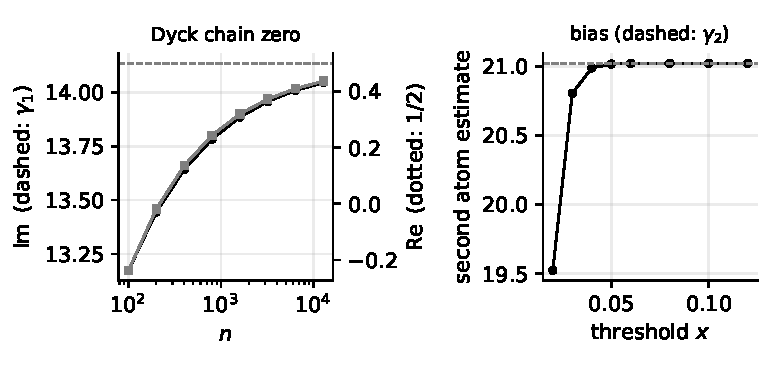
\includegraphics[width=\textwidth]{fig/ev_smith_tawn.pdf}
\caption{Left: real and imaginary part of the zero of the Dirichlet polynomial of the Dyck chain near $\gamma_1$ for $n=100$ to $12800$ (dashed: $\gamma_1$, dotted: the real part $\tfrac12$). Right: estimate of the second atom of the hitting time law after deflating the first, against the threshold $x$ (dashed: $\gamma_2$).}\label{ev:fig:st}
\end{figure}

\section{Hitting times and the Thorin variable}\label{ev:sec:kent}

Kent's theorem and Krein's converse (Proposition~\ref{ht:prop:kent}, Section~\ref{sec:ch18:kent}; Kent \cite{Kent80}, Dym and McKean \cite{DymMcKean76}, and for generalised diffusions Kotani and Watanabe \cite{KotaniWatanabe82} and Knight \cite{Knight81}) are used in the following form. A string with a reflecting end and a Dirichlet end has simple spectrum, so the converse holds only for strictly increasing sequences $0<\lambda_1<\lambda_2<\cdots$ with $\sum_k\lambda_k^{-1}<\infty$. And the string is not unique: the hitting time law fixes the eigenvalues and not the norming constants (a string with two point masses has three parameters modulo the natural scale and two eigenvalues, so a one parameter family has the same hitting time law). The spectral measure, eigenvalues together with weights, is what determines the string by Krein's algorithm.
% UNCHECKED: KotaniWatanabe82, Knight81, the statement is the source's and the paper was not read for this book.

Let $\widehat H$ be an even real entire function of order less than two with $\widehat H(0)>0$, and put
\[
\widehat L(s) = \frac{\widehat H(0)}{\widehat H(2i\sqrt s)} ,
\]
which for $\widehat H=H$ is $L(s)=\xi(\tfrac12)/\xi(\tfrac12+\sqrt s)=\prod_k(1+s/\gamma_k^2)^{-1}$. Because the order is below two, $\widehat H(2i\sqrt s)$ has order below one in $s$ and is the canonical product of genus zero over its zeros. Here $\pm\gamma_k$ are the zeros of $\Xi$, real exactly when the zeros of $\zeta$ lie on the critical line, in which case $0<\gamma_1\le\gamma_2\le\cdots$.

\begin{corollary}\label{ev:cor:rh}
Write $\pm\gamma_k$ for the zeros of $\Xi$, ordered by real part, so that $\frac12+i\gamma_k$ are the nontrivial zeros of $\zeta$ (the $\gamma_k$ are ordinates, real under RH). The following are equivalent.
\begin{enumerate}
\item All zeros of $\Xi$ are real (RH).
\item $L$ is the Laplace transform of a generalised gamma convolution whose Thorin measure $\sum_k\delta_{\gamma_k^2}$ is positive (Polson \cite{P17}, Proposition~\ref{prop:rigid}).
\end{enumerate}
Moreover, all zeros of $\Xi$ are real and simple if and only if there is a Krein string with positive mass whose hitting time $T$ satisfies $\E e^{-sT}=L(s)$. The same statements hold with $\widehat H$ and $\widehat L$ in place of $H$ and $L$.
\end{corollary}

\begin{proof}
The equivalence of (1) and (2) is Proposition~\ref{prop:rigid} and Theorem~\ref{mw:thm:stieltjes}. If the zeros are real and simple, the $\gamma_k^2$ are strictly increasing and Krein's converse gives a string. If a string exists, its spectrum is real, positive and simple, and by Kent's theorem $\E e^{-sT}=\prod_k(1+s/\lambda_k)^{-1}$; the zeros of $\widehat H(2i\sqrt s)$ in $s$ are then the $-\lambda_k$, so the zeros of $\widehat H$ are real and simple. The same argument covers $\widehat H$.
\end{proof}

So the zeros are real and simple exactly when the string exists (Proposition~\ref{ht:prop:kent} also assumes simple zeros; simplicity of the zeros of $\Xi$ is not known). Two features of the string are visible without exhibiting it.

\begin{proposition}[Principal eigenvalue from the tail]\label{ev:prop:tail}
If RH holds, the zeros are simple and $|\xi'(\rho)|\ge e^{-C|\gamma|}$ for some constant $C$ and all zeros $\rho=\frac12+i\gamma$ (the hypothesis of Theorem~\ref{ht:thm:res}), then $\mathbb{P}(T > x) = \sum_k c_ke^{-\gamma_k^2x}$ with $c_k = \prod_{j\ne k}(1 - \gamma_k^2/\gamma_j^2)^{-1} = 2i\xi(\tfrac12)/(\gamma_k\xi'(\tfrac12 + i\gamma_k))$. In particular the excess of $T$ over a high threshold is asymptotically exponential with rate $\lambda_1 = \gamma_1^2$, the bottom of the spectrum of the string; this last clause needs only the two term tail of Proposition~\ref{ht:prop:tail}, which has no hypothesis on $\xi'$.
\end{proposition}

This is Proposition~\ref{ht:prop:tail} and the hazard rate of Section~\ref{sec:ch18:law} in the present notation. The exponential excess follows from the expansion and is analogous to the peaks over threshold theorem of Pickands and of Balkema and de Haan \cite{Pickands75,BalkemaDeHaan74}, which is not used. The estimator is the hazard rate. At a threshold $x$ the ratio of the density to the tail, $f(x)/\mathbb{P}(T>x)$, tends to $\gamma_1^2$, and the Laplace inversion of $L$ (the method of Talbot, at $100$ and $130$ nodes, agreeing to $20$ digits) uses no zero. On the window $x\in[0.18,0.20]$ the square root of this ratio is $14.1347251417346937\ldots$ at all three of $x=0.18,0.19,0.20$ (the values are $14.13472514173469373756$, $\ldots3785760$ and $\ldots3790040$ against $\gamma_1=14.13472514173469379045\ldots$), so $\gamma_1$ is recovered to eighteen significant digits (computed). The threshold bias for the later atoms is the point of Smith and Tawn: deflating by the first atom, the second atom is estimated as $21.0167$, $21.0212$ and $21.02204$ from the thresholds $x=0.05$, $0.06$ and $0.1$, against $\gamma_2=21.02204$ (computed). Figure~\ref{ev:fig:tail} shows the error of these estimates of $\gamma_1$.
% UNCHECKED: Pickands75, BalkemaDeHaan74, the statement is the source's and the paper was not read for this book.

\begin{figure}[h]\centering
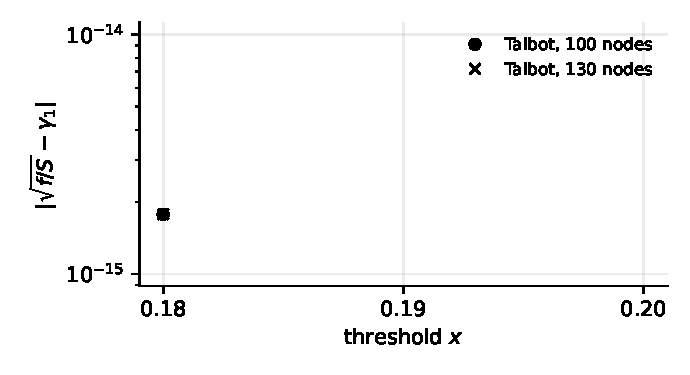
\includegraphics[width=0.9\textwidth]{fig/ev_tail.pdf}
\caption{Error of the estimate $\sqrt{f(x)/\mathbb{P}(T>x)}$ of $\gamma_1$ from the Laplace inversion of $L$ (Talbot, $100$ and $130$ nodes) at $x=0.18,0.19,0.20$.}\label{ev:fig:tail}
\end{figure}

\section{B splines, Hadamard products and Thorin}\label{ev:sec:bspline}

Is there a B spline view of the Gumbel law that leads to a Hadamard product and from there to a Thorin representation? The first two steps are known. By R\'enyi's representation the maximum of $n$ independent exponentials is $M_n=\sum_{k\le n}E_k/k$, a generalised gamma convolution with Thorin measure $\sum_{k\le n}\delta_k$ and the passage time of a pure death chain; $M_n-\log n$ tends to the Gumbel law $G$, with $\E e^{-sG}=\Gamma(1+s)=\exp\big(-\gamma_Es-\sum_{k\ge1}[\log(1+s/k)-s/k]\big)$, a compensated Thorin representation with atoms at the integers (the compensation is needed because $\sum1/k$ diverges and is what the centring $\log n$ removes). The density of $M_n$ is, up to the factor $y^{n-1}$ and a Laplace transform, a B spline with the knots $1,\ldots,n$, and the same holds for the truncations of the reciprocal $\xi$ law with knots $\gamma_1^2,\ldots,\gamma_K^2$ (Proposition~\ref{ht:prop:bspline} and Section~\ref{ht:sec:ev}, which also give the Dirichlet mean form; the density of a sum of exponentials is the divided difference of $e^{-\lambda x}$ in $\lambda$, which is the B spline only after this transform). If RH holds, the truncated laws shifted by the tail mean $r_K=\sum_{k>K}\gamma_k^{-2}$ converge to the reciprocal $\xi$ law, since the difference has mean zero and variance $\sum_{k>K}\gamma_k^{-4}\to0$; no compensation is needed because $\sum_k\gamma_k^{-2}<\infty$ (the shift is the tail shift of the Kent approximants of Section~\ref{sec:ch18:kent}).

Figure~\ref{ev:fig:bspline} shows the supremum distances against $K$. For the reciprocal $\Xi$ law the supremum distance between the shifted truncation and the density obtained by Laplace inversion is $128$ and $42$ for $K=1,2$ (attained at the knot $r_K$, where the truncated density jumps or ends), and $8.1$, $0.80$ and $0.23$ for $K=5,20,40$, against a peak density of $80$ (computed; on a uniform grid of mesh $5\cdot10^{-4}$, which misses the knot, they are $110$ and $36$, and the source printed $114$ and $37$).

\begin{figure}[h]\centering
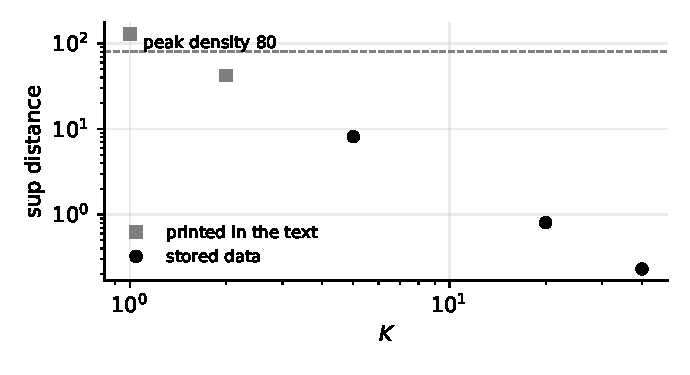
\includegraphics[width=\textwidth]{fig/ev_bspline.pdf}
\caption{Supremum distance between the mean corrected truncation with knots $\gamma_1^2,\ldots,\gamma_K^2$ and the density of the reciprocal $\Xi$ law, against $K$ (dashed: the peak density $80$). The values for $K=5,20,40$ are stored data, those for $K=1,2$ are the printed values above.}\label{ev:fig:bspline}
\end{figure}

For the P\'olya density the B spline view gives the following.
\begin{enumerate}
\item Each Gumbel piece of Theorem~\ref{ev:thm:decomp} has its own exact chain. The piece $g_k$ is the law of $-\log G_k$, so $\E e^{-sX}=\E G_k^s=\Gamma(k+s)/\Gamma(k)$, and the Weierstrass product gives a compensated Thorin form with atoms at $k,k+1,k+2,\ldots$. For the P\'olya pieces these are $\tfrac94+j$ and $\tfrac54+j$ (proved).
\item In $\xi(s) = \tfrac12s(s-1)\pi^{-s/2}\Gamma(s/2)\zeta(s)$ this Gumbel structure is the archimedean factor $\Gamma(s/2)$. Its poles are at $s=0,-2,-4,\ldots$; the pole at $0$ is cancelled by the factor $s$ and the others by the trivial zeros $-2,-4,\ldots$ of $\zeta$, so the knots of the Gumbel view correspond to the trivial zeros (proved).
\item The atoms at $\gamma_k^2$ do not come from any product of Gumbel pieces. They come from the theta superposition $\Phi=\sum_n\phi_n$, which translates one Gumbel kernel along the lattice $\tfrac12\log n$ and turns the Gamma factor into $\Gamma(s/2)\zeta(s)$ (Theorem~\ref{ev:thm:decomp}). A superposition is a sum, not a product, and a sum does not preserve Hadamard products or Thorin form (a heuristic remark: it explains why the argument stops, and proves nothing).
\end{enumerate}
So the B spline view leads to a Hadamard product and a Thorin representation for every Gumbel piece unconditionally and for the reciprocal $\Xi$ law given the zeros. The step that would make it a route to RH, that the superposition of Gumbel pieces still has a positive Thorin measure, is the open question of this chapter in another form.

\section{An explicit string: the Liouville operator}\label{ev:sec:liouville}

P\'olya proved that his two sided kernels have only real zeros \cite{Polya15,Polya}; the spectral reading is Titchmarsh's \cite{TitchmarshEigen46} and the hitting time form Biane's \cite{Biane09} (Section~\ref{ch:biane}). For $a>0$ the function $g(\tau)=K_\nu(ae^\tau)$ solves $g''-a^2e^{2\tau}g=\nu^2g$, the real zeros $z_k$ of $z\mapsto K_{iz}(a)$ are the square roots of the Dirichlet eigenvalues of $-g''+a^2e^{2\tau}g$ on $(0,\infty)$ with $g(0)=0$, and the diffusion obtained by the Doob transform of this operator by its positive solution $K_0(ae^\tau)$, started at the entrance boundary at $+\infty$, has hitting time $T_0$ of $0$ with
\[
\E e^{-sT_0}=\frac{K_0(a)}{K_{\sqrt s}(a)}=\prod_k\Big(1+\frac s{z_k^2}\Big)^{-1}
\]
(Proposition~\ref{prop:biane:liouville} and Theorem~\ref{thm:biane:clock}, proved, with simple spectrum). The product form uses that $K_{\sqrt s}(a)$ has order one half in $s$, because $|K_\nu(a)|\le K_{|\operatorname{Re}\nu|}(a)\le C\,\Gamma(|\nu|+1)(2/a)^{|\nu|}$, so Hadamard's factorisation has genus zero with no exponential factor.

A second order finite difference discretisation of the operator on $(0,6)$ with $a=2\pi$ and about $64000$ intervals (the size at which the digits of the source are reproduced) gives $\sqrt{\lambda_k}=9.768770$, $12.448488$, $14.684960$, $16.691578$, $18.549374$, and the zeros of $K_{iz}(2\pi)$ are $9.768770$, $12.448488$, $14.684960$, $16.691579$, $18.549375$ (computed; with certified signs of the Bessel values, bisection gives $9.76877008$, $12.44848789$, $14.68495978$, $16.69157894$, $18.54937520$).

P\'olya's kernel involves $K_{(9\pm iz)/4}(2\pi)$, not $K_{iz}(2\pi)$; he passes between them with the shift lemma: if $G$ is real entire of genus at most one with only real zeros, so is $\tfrac12[G(z+ic)+G(z-ic)]$, which is the transform of $\cosh(cu)$ times the original kernel. The lemma deals with one Bessel term, and the combination of the two terms of $\Phi^P$ is handled in the refinement of Section~\ref{pol:sec:papers} (which also records that the kernel with the second exponential term kept is real rooted). The lemma preserves real zeros, hence by Corollary~\ref{ev:cor:rh} the existence of a string when the zeros are simple, but does not say what the new string is; writing it explicitly is Problem~2 of Section~\ref{ev:sec:work}.

\section{The string test from kernel moments}\label{ev:sec:string}

For a general approximation the string is not known, but whether the zeros are real, the first condition for it to exist, can be tested from the kernel alone. Expand
\[
\begin{aligned}
\widehat H(2i\sqrt s) &= \int_0^\infty\widehat\Phi(u)\cosh(2\sqrt s\,u)\,du = \sum_{m\ge0}\frac{4^m M_{2m}}{(2m)!}s^m,\\
M_{2m} &= \int_0^\infty u^{2m}\widehat\Phi(u)\,du .
\end{aligned}
\]
Taking logarithms gives $\log[\widehat H(2i\sqrt s)/\widehat H(0)]=\sum_j(-1)^{j+1}\mu_js^j/j$ with
\[
\mu_j = \sum_k\widehat\gamma_k^{-2j},
\]
the power sums of the inverse Thorin atoms, equivalently $\kappa_j(T)/(j-1)!$ for the cumulants $\kappa_j(T)$ of the candidate hitting time. Put $w_k=\widehat\gamma_k^{-2}$ and $\nu=\sum_kw_k\delta_{w_k}$, so that $\mu_{j+1}=\int y^j\nu(dy)$ whenever the $w_k$ are positive.

\begin{proposition}[Hankel test]\label{ev:prop:hankel}
Let $\widehat H$ be as in Section~\ref{ev:sec:kent}, with infinitely many zeros and $\sum_k|w_k|<\infty$. The zeros of $\widehat H$ are all real (and nonzero) if and only if all the Hankel determinants
\[
D_n = \det[\mu_{i+j+1}]_{i,j=0}^{n-1}, \qquad D_n' = \det[\mu_{i+j+2}]_{i,j=0}^{n-1}, \qquad n\ge1,
\]
are positive.
\end{proposition}

\begin{proof}
If the zeros are real, $\nu$ is a positive measure on $(0,\infty)$ and the determinants are those of the Stieltjes moment problem, hence positive. Conversely, if all are positive, the sequence $(\mu_{j+1})$ is a Stieltjes moment sequence. It grows at most like $\rho^j$ with $\rho=\max_k|w_k|$, so the representing measure $\nu'$ is unique and supported in $[0,\rho]$, and its Stieltjes transform $\int\nu'(dy)/(1-zy)$ is analytic off $[1/\rho,\infty)$ and equals $\sum_{j\ge0}\mu_{j+1}z^j$ near $0$. That series is also $\sum_kw_k/(1-zw_k)$, a meromorphic function (the sum converges locally uniformly off the poles because $\sum|w_k|<\infty$) with poles exactly at the points $1/w_k$ and residues that do not cancel, since terms with equal $w_k$ add with the same sign and distinct $w_k$ give distinct poles. By analytic continuation the poles lie in $[1/\rho,\infty)$, so every $w_k$ is real and positive.
\end{proof}

The continued fraction coefficients built from $D_n$ and $D_n'$ are the masses and lengths of a discrete string, a birth and death chain whose hitting time matches the first $2n$ cumulants (classical, Stieltjes and Krein; the wording of the matching was not checked). % UNCHECKED: the statement that the discrete string of order n matches exactly the first 2n cumulants is quoted from the source and from the classical continued fraction theory; it was not rederived.
So the test is a hitting time calculation: build the chain and check that its rates are positive. It is a finite form of the Stieltjes criterion of Theorem~\ref{mw:thm:stieltjes}, and the moment matching along the Kent approximants is in Section~\ref{sec:ch18:moments}.

The moments $M_{2m}$ were computed by quadrature for the exact kernel, the two term folded kernel and P\'olya's two term kernel, then $\mu_j$, then $D_n$ and $D_n'$. At $180$ digits all of $D_1,\ldots,D_{11}$ and $D_1',\ldots,D_{11}'$ are positive for all three kernels, with the sign of each determinant certified by ball arithmetic from the computed moments (the quadrature error of the moments is not certified; the relative change between two node counts is below $10^{-89}$; computed). For example $D_{11}=8.99\cdot10^{-368}$ for the exact kernel, $9.52\cdot10^{-368}$ for the folded kernel and $1.14\cdot10^{-350}$ for P\'olya's, and $D_6=8.1\cdot10^{-100}$ for the exact kernel. The first moment is $\mu_1=\sum_k\gamma_k^{-2}=0.0231049931154190$ for the exact kernel, which equals $\xi''(\tfrac12)/(2\xi(\tfrac12))$ computed independently by a Cauchy integral; for the two term folded kernel it is $0.0231049931181204$, and for P\'olya's kernel $0.0363173599127934$.

The positive result for the folded kernel, which has nonreal zeros above height about $x=40$ (Table~\ref{ev:tab:approx}), shows the limitation of the test. A Hankel matrix of order $n$ sees roughly the first $n$ atoms, and the weights of the atoms decay like $\widehat\gamma^{-2j}$, so an off line pair at height $x$ needs an order beyond the number of real atoms below $x$, and precision of the order of $4n\log_{10}(x/\gamma_1)$ digits, before it can make a determinant negative (heuristic; the masking of the first pair is measured in Section~\ref{ev:sec:round2}). Finite order positivity certifies a positive string for a truncated moment problem, which is the analogue of verifying RH to a finite height, and it mirrors Li's criterion \cite{Li97}, where finitely many positive coefficients prove nothing about RH.
